\chapter{Assessment of Renal $T_2$ Mapping Methods}
\label{chap:t2_mapping}

\begin{abstract}
	This work was presented as an aural presentation at the \ac{ISMRM} 28th Annual Meeting (2020) \cite{daniel_comparison_2020}.\\
	\lipsum[1]
\end{abstract}
\newpage

\section{Introduction}
\label{sec:t2_intro}



\section{Methods}
\label{sec:t2_methods}

\subsection{Theory}

There are multiple methods for acquiring $T_2$ maps in the kidneys, \ac{SE}-\ac{EPI}, \ac{ME-TSE}, \ac{GraSE} and $T_2$ preparation. We wish to compare each of these methods in-vivo and verify their accuracy using a calibrated phantom. A QalibreMD System Standard Model 130 \cite{noauthor_system_nodate} is used for verification. All data is collected on a Philips 3T Ingenia system. 

\begin{figure}[H]
	\centering
	\includegraphics[width=0.5\textwidth]{T2_Mapping/Phantom_Example/T2_Spheres.eps}
	\caption{A schematic of the $T_2$ spheres in the QalibreMD phantom.}
	\label{fig:t2_phantom_schematic}	
\end{figure}

\subsection{Spin Echo-Echo Planar Imaging}
A series of volumes are collected at a range of echo times using a multi-slice spin echo acquisition with \ac{EPI} readout. Acquisition parameters are \ac{FOV} = 288 $\times$ 288 $\times$ 25 mm, voxel size = 3 $\times$ 3 $\times$ 5 mm$^3$, \ac{TR} = 5000 ms, \ac{FA} = $90\degree$, \ac{SENSE} = 2.55, halfscan = 0.844 and the sequence is respiratory triggered for in-vivo use and has an acquisition time of approximately 9 minutes depending on breathing rate. Volumes are acquired at \ac{TE} between 20 ms and 70 ms in 5 ms steps with four volumes being acquired at each echo time. 

\begin{figure}[H]
	\centering
	\includegraphics[width=0.95\textwidth]{T2_Mapping/Pulse_Diagrams/SE-EPI/SE-EPI_Sequence-01.eps}
	\caption{A pulse sequence diagram of the \ac{SE}-\ac{EPI} scheme.}
	\label{fig:t2_se-epi_seq}	
\end{figure}

\subsection{Multi-Echo Turbo Spin Echo}

This method also uses a multi-slice spin echo acquisition however unlike the simple spin echo method, uses a multishot \ac{TSE} readout. Acquisition parameters for in-vivo scanning are \ac{FOV} = 288 $\times$ 288 $\times$ 25 mm, voxel size = 3 $\times$ 3 $\times$ 5 mm$^3$, \ac{TR} = 3000 ms, \ac{FA} = $90\degree$, \ac{SENSE} = 2.55 and \ac{TSE} factor = 10; the sequence is respiratory triggered and has an acquisition time of approximately 4 minutes depending on breathing rate. For phantom scanning, the following parameters are modified \ac{FOV} = 250 $\times$ 250 $\times$ 6 mm, voxel size = 0.9 $\times$ 0.9 $\times$ 6 mm$^3$ and respiratory triggering is removed. Volumes are collected with \ac{TE} between 13 ms and 130 ms in 13 ms steps.

\begin{figure}[H]
	\centering
	\includegraphics[width=0.95\textwidth]{T2_Mapping/Pulse_Diagrams/ME-TSE/ME-TSE_Sequence-01.eps}
	\caption{A pulse sequence diagram of the \ac{ME-TSE} scheme.}
	\label{fig:t2_me-tse_seq}	
\end{figure}

\subsection{Gradient Spin Echo}

This method also uses a multi-slice spin echo acquisition but with a \ac{GraSE} readout. Acquisition parameters for in-vivo scanning are \ac{FOV} = 288 $\times$ 288 $\times$ 25 mm, voxel size = 3 $\times$ 3 $\times$ 5 mm$^3$, \ac{TR} = 3000 ms, \ac{FA} = $90\degree$, \ac{SENSE} = 2.55 and \ac{TSE} factor = 30, startup echoes = 1; the sequence is respiratory triggered and has an acquisition time of approximately 5 minutes depending on breathing rate. For phantom scanning, the following parameters are modified \ac{FOV} = 250 $\times$ 250 $\times$ 6 mm, voxel size = 0.9 $\times$ 0.9 $\times$ 6 mm$^3$ and respiratory triggering is removed. Volumes are collected with \ac{TE} between 11.2 ms and 173.3 ms in 5.6 ms steps.

\begin{figure}[H]
	\centering
	\includegraphics[width=0.95\textwidth]{T2_Mapping/Pulse_Diagrams/GraSE/GraSE_Sequence-01.eps}
	\caption{A pulse sequence diagram of the \ac{GraSE} scheme.}
	\label{fig:t2_grase_seq}	
\end{figure}

\subsection{$T_2$ Preperation}

\subsubsection{Basic $T_2$ Preperation}

\begin{figure}[H]
	\centering
	\includegraphics[width=0.95\textwidth]{T2_Mapping/Pulse_Diagrams/Philips_T2_Prep/T2_Prep_Sequence-01.eps}
	\caption{A pulse sequence diagram of the basic $T_2$ preparation scheme.}
	\label{fig:t2_t2prep_seq}	
\end{figure}

\subsubsection{CPMG $T_2$ Preparation}

This technique uses a multi-slice \ac{FFE} acquisition with a \ac{TFEPI} readout. Varying degrees of $T_2$ weighting are applied as a series of $180\degree$ preparation pulses for a variable \ac{eTE}, this is similar to the sequence used in Section \ref{sec:TRUST_MRI}. Acquisition parameters for in-vivo scanning are \ac{FOV} = 288 $\times$ 288 $\times$ 25 mm, voxel size = 3 $\times$ 5.65 $\times$ 5 mm$^3$ (voxel size is limited by the \ac{EPI} factor), \ac{TR} = 3000 ms, \ac{TE} = 5.3, \ac{FA} = $90\degree$, \ac{EPI} factor = 17, \ac{SENSE} = 3 and halfscan = 0.733; the sequence is respiratory triggered and has an acquisition time of approximately 6 minutes depending on breathing rate. As the voxel size is already at its minimum, the only modifications made for scanning the phantom are to decrease the \ac{FOV} to 250 $\times$ 250 $\times$ 6 mm and remove respiratory triggering. \ac{eTE}s of 0, 40, 80 and 160 ms are used with three volumes acquired at each \ac{eTE}

\begin{figure}[H]
	\centering
	\includegraphics[width=0.95\textwidth]{T2_Mapping/Pulse_Diagrams/CPMG_T2_Prep/CPMG_T2_Prep_Sequence-01.eps}
	\caption{A pulse sequence diagram of the \ac{CPMG} $T_2$ preperation scheme.}
	\label{fig:t2_cpmg_t2prep_seq}	
\end{figure}

\subsection{Adaptations for In-Vivo Use}

\subsection{Analysis}

The data is fit on a voxel by voxel basis using a least squares trust region reflective method to fit the data to Equation \eqref{eq:T2} to estimate $T_2$ and $S_0$ with an uncertainty in the fit \cite{branch_subspace_1999}. For methods where multiple volumes are acquired at an \ac{TE}, individual volumes are used for the fit e.g. four points at each \ac{TE} for the \ac{SE}-\ac{EPI} method rather than taking the mean of the volumes for each \ac{TE}, this makes potential data discarding easier. This post-processing is performed by an in-house Python package. Once the $T_2$ maps have been generated, \ac{ROI} can be defined for different tissue types or phantom compositions.

\begin{equation}
S(t) = S_0 \cdot e^{-t/T_2}
\label{eq:T2}
\end{equation}

\section{Results}

\subsubsection{Quantitative Phantom}

We began by comparing the quantitative accuracy of each of the proposed $T_2$ mapping methods (spin echo \ac{EPI}, multi-echo \ac{TSE}, \ac{GraSE} and $T_2$ preparation).  The QalibreMD System Standard Model 130 phantom used has fourteen spheres with $T_2$ between 5.35 ms and 645.8 ms spanning the range of $T_2$ expected in the kidneys, Figure \ref{fig:t2_phantom_eg}. This phantom was scanned using each of the methods outlined in \ref{sec:t2_methods} and a \ac{ROI} defined for each sphere. 

\begin{figure}[H]
	\centering
	\begin{subfigure}[c]{0.47\textwidth}
		\centering
		\includegraphics[width=1\textwidth]{T2_Mapping/Phantom_Example/Localiser_multi.eps}
		\caption{}
		\label{fig:t2_phantom_loc}
	\end{subfigure}
	\hfill
	\begin{subfigure}[c]{0.47\textwidth}
		\centering
		\includegraphics[width=1\textwidth]{T2_Mapping/Phantom_Example/GraSE_map_0_500.eps}
		\caption{}
		\label{fig:t2_phantom_map}
	\end{subfigure}
	\caption{(\subref{fig:t2_phantom_loc}) The $T_2$ spheres inside the phantom. (\subref{fig:t2_phantom_map}) An example $T_2$ map, in this case generated using the \ac{GraSE} method.}
	\label{fig:t2_phantom_eg}
\end{figure}

The spin echo method produced vastly over-estimated readings for the spheres of $T_2$ less than 20 ms (Figures \ref{fig:t2_phantom_se_mean}) due to the longer minimum \ac{TE} compared to the other methods. This can be seen in Figure \ref{fig:t2_phantom_se_raw} where the signal from the shortest $T_2$ spheres has already mostly decayed. This method did however deliver accurate measurements for the remaining spheres.\\

More accurate results were generated for shorter $T_2$ spheres using the \ac{ME-TSE} method. The raw data (Figure \ref{fig:t2_phantom_metse_raw}) is more noisy, with a sawtooth pattern visible, this additional noise manifests itself as inaccuracies in the longer $T_2$ measurements where the dynamic range over the \ac{TE} sampled is smaller.\\

The \ac{GraSE} method produced the most accurate measurements although still struggled to measure the sphere with a $T_2$ of 5.35 ms, Figure \ref{fig:t2_phantom_grase_mean}. The large range of \ac{TE} and number of volumes collected means this method produced the most accurate results. It also has the benefit of being able to be performed at high resolutions with voxel sizes of 0.9 x 0.9 mm unlike the \ac{SE}-\ac{EPI} and $T_2$ prep methods; this makes it well suited to both in-vivo and ex-vivo measurements.\\

The data collected using the $T_2$ prep method (Figures \ref{fig:t2_phantom_t2prep_raw} and \ref{fig:t2_phantom_t2prep_mean}) did not fit well due to its small number of data points and large degradation in image quality.\\

\begin{figure}[H]
	\centering
	\begin{subfigure}[c]{0.9\textwidth}
		\centering
		\begin{subfigure}[c]{0.47\textwidth}
			\centering
			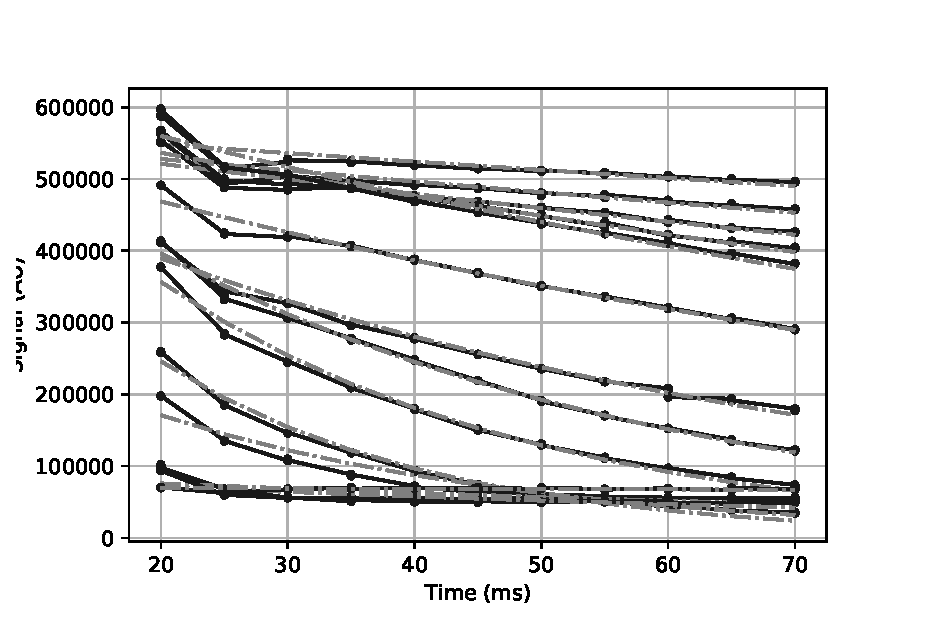
\includegraphics[width=1\textwidth]{T2_Mapping/Phantom/SE_raw.eps}
			\caption{}
			\label{fig:t2_phantom_se_raw}
		\end{subfigure}
		\hfill
		\begin{subfigure}[c]{0.47\textwidth}
			\centering
			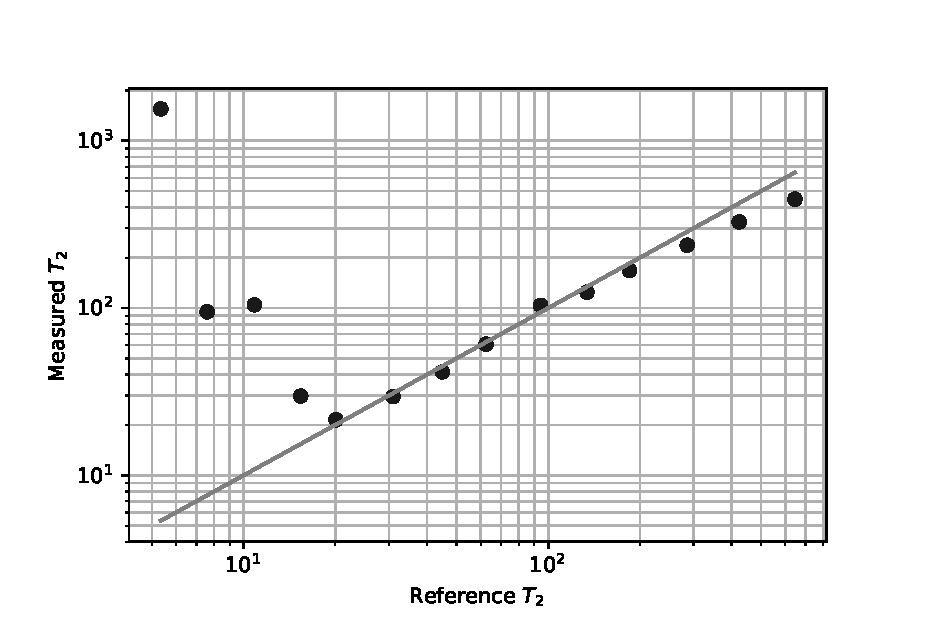
\includegraphics[width=1\textwidth]{T2_Mapping/Phantom/SE_mean.eps}
			\caption{}
			\label{fig:t2_phantom_se_mean}
		\end{subfigure}
	\end{subfigure}
	\vskip\baselineskip
	\begin{subfigure}[c]{0.9\textwidth}
		\centering
		\begin{subfigure}[c]{0.47\textwidth}
			\centering
			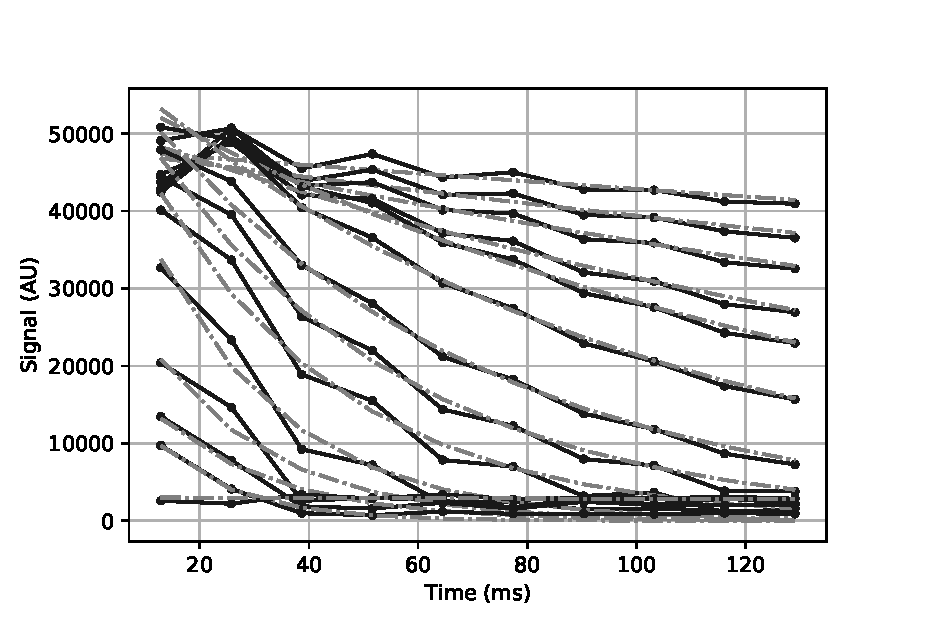
\includegraphics[width=1\textwidth]{T2_Mapping/Phantom/METSE_HR_raw.eps}
			\caption{}
			\label{fig:t2_phantom_metse_raw}
		\end{subfigure}
		\hfill
		\begin{subfigure}[c]{0.47\textwidth}
			\centering
			\includegraphics[width=1\textwidth]{T2_Mapping/Phantom/METSE_HR_mean.eps}
			\caption{}
			\label{fig:t2_phantom_metse_mean}
		\end{subfigure}
	\end{subfigure}
	\vskip\baselineskip
	\begin{subfigure}[c]{0.9\textwidth}
		\centering
		\begin{subfigure}[c]{0.47\textwidth}
			\centering
			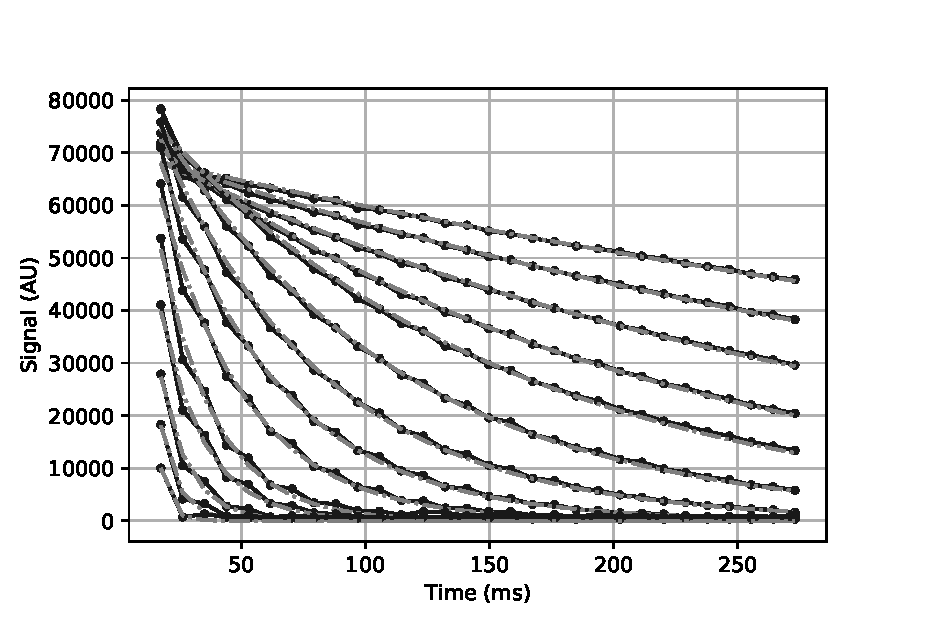
\includegraphics[width=1\textwidth]{T2_Mapping/Phantom/GraSE_HR_raw.eps}
			\caption{}
			\label{fig:t2_phantom_grase_raw}
		\end{subfigure}
		\hfill
		\begin{subfigure}[c]{0.47\textwidth}
			\centering
			\includegraphics[width=1\textwidth]{T2_Mapping/Phantom/GraSE_HR_mean.eps}
			\caption{}
			\label{fig:t2_phantom_grase_mean}
		\end{subfigure}
	\end{subfigure}
	\vskip\baselineskip
	\begin{subfigure}[c]{0.9\textwidth}
		\centering
		\begin{subfigure}[c]{0.47\textwidth}
			\centering
			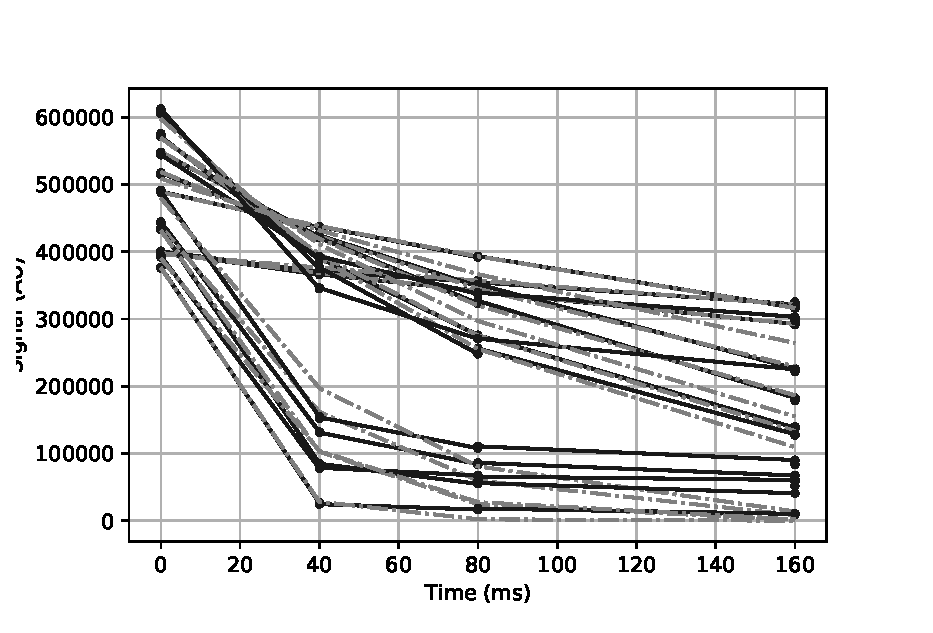
\includegraphics[width=1\textwidth]{T2_Mapping/Phantom/T2prep_raw.eps}
			\caption{}
			\label{fig:t2_phantom_t2prep_raw}
		\end{subfigure}
		\hfill
		\begin{subfigure}[c]{0.47\textwidth}
			\centering
			\includegraphics[width=1\textwidth]{T2_Mapping/Phantom/T2prep_mean.eps}
			\caption{}
			\label{fig:t2_phantom_t2prep_mean}
		\end{subfigure}
	\end{subfigure}
	\caption{Figures (\subref{fig:t2_phantom_se_raw}), (\subref{fig:t2_phantom_metse_raw}), (\subref{fig:t2_phantom_grase_raw}) and (\subref{fig:t2_phantom_t2prep_raw}) show the raw signal decay for each of the fourteen spheres and the fit decay. Figures (\subref{fig:t2_phantom_se_mean}), (\subref{fig:t2_phantom_metse_mean}), (\subref{fig:t2_phantom_grase_mean}) and (\subref{fig:t2_phantom_t2prep_mean}) show how the fit $T_2$ compares to the literature value. Figures (\subref{fig:t2_phantom_se_raw}) and (\subref{fig:t2_phantom_se_mean}) show the results from the \ac{SE}-\ac{EPI} method, (\subref{fig:t2_phantom_metse_raw}) and (\subref{fig:t2_phantom_metse_mean}) show the results form the \ac{ME-TSE} method, (\subref{fig:t2_phantom_grase_raw}) and (\subref{fig:t2_phantom_grase_mean}) show the results form the \ac{GraSE} method and (\subref{fig:t2_phantom_t2prep_raw}) and (\subref{fig:t2_phantom_t2prep_mean}) show the results from the $T_2$ prep method.} 
	\label{fig:t2_phantom}
\end{figure}


\subsubsection{In-Vivo}

$T_2$ maps using all four methods were collected on the same subject in the same scanning session to allow for a direct comparison of the in-vivo data.\\ 

\begin{figure}[H]
	\centering
	\begin{subfigure}[c]{0.9\textwidth}
		\centering
		\begin{subfigure}[c]{0.47\textwidth}
			\centering
			\includegraphics[width=1\textwidth]{T2_Mapping/SE/SE_Raw_Echoes.eps}
			\caption{}
			\label{fig:t2_t2_se_raw}
		\end{subfigure}
		\hfill
		\begin{subfigure}[c]{0.47\textwidth}
			\centering
			\includegraphics[width=1\textwidth]{T2_Mapping/SE/SE_Map.eps}
			\caption{}
			\label{fig:t2_t2_se_map}
		\end{subfigure}
	\end{subfigure}
	\vskip\baselineskip
	\begin{subfigure}[c]{0.9\textwidth}
		\centering
		\includegraphics[width=1\textwidth]{T2_Mapping/SE/SE_Decay.eps}
		\caption{}
		\label{fig:t2_t2_se_decay}			
	\end{subfigure}
	\caption{(\subref{fig:t2_t2_se_raw}) The raw data used to generate the \ac{SE}-\ac{EPI} $T_2$ map.  (\subref{fig:t2_t2_se_map}) An example slice from the \ac{SE}-\ac{EPI} $T_2$ map. (\subref{fig:t2_t2_se_decay}) The signal decay for the renal cortex and medulla.} 
	\label{fig:t2_t2_se}
\end{figure}

The \ac{SE}-\ac{EPI} method (Figure \ref{fig:t2_t2_se}) generated maps with little blurring however there is also a lack of differentiation in $T_2$ between the renal cortex and medulla. The data collected at \ac{TE} of 20 ms appears to be artificially high and leads to a reduction in fit $T_2$. This sequence is the most susceptible of the methods to patient motion due to the acquisition method of a series per \ac{TE}, this increase in motion is clear when scrolling through \ac{TE}. 

\begin{figure}[H]
	\centering
	\begin{subfigure}[c]{0.9\textwidth}
		\centering
		\begin{subfigure}[c]{0.47\textwidth}
			\centering
			\includegraphics[width=1\textwidth]{T2_Mapping/ME/ME_Raw_Echoes.eps}
			\caption{}
			\label{fig:t2_t2_me_raw}
		\end{subfigure}
		\hfill
		\begin{subfigure}[c]{0.47\textwidth}
			\centering
			\includegraphics[width=1\textwidth]{T2_Mapping/ME/ME_Map.eps}
			\caption{}
			\label{fig:t2_t2_me_map}
		\end{subfigure}
	\end{subfigure}
	\vskip\baselineskip
	\begin{subfigure}[c]{0.9\textwidth}
		\centering
		\includegraphics[width=1\textwidth]{T2_Mapping/ME/ME_Decay.eps}
		\caption{}
		\label{fig:t2_t2_me_decay}			
	\end{subfigure}
	\caption{(\subref{fig:t2_t2_me_raw}) The raw data used to generate the \ac{ME-TSE} $T_2$ map.  (\subref{fig:t2_t2_me_map}) An example slice from the \ac{ME-TSE} $T_2$ map. (\subref{fig:t2_t2_me_decay}) The signal decay for the renal cortex and medulla.} 
	\label{fig:t2_t2_me}
\end{figure}

The map generated by the \ac{ME-TSE} method (Figure \ref{fig:t2_t2_me}) suffers from a large amount of blurring due to the relatively long echo train length. The number of echoes acquired is limited to the \ac{TSE} factor therefore to acquire ten echoes, a \ac{TSE} factor of ten needs to be used. This blurring leads to structures being obscured in the map and only a very small differentiation between cortex and medulla.

\begin{figure}[H]
	\centering
	\begin{subfigure}[c]{0.9\textwidth}
		\centering
		\begin{subfigure}[c]{0.47\textwidth}
			\centering
			\includegraphics[width=1\textwidth]{T2_Mapping/GraSE/GraSE_Raw_Echoes.eps}
			\caption{}
			\label{fig:t2_t2_grase_raw}
		\end{subfigure}
		\hfill
		\begin{subfigure}[c]{0.47\textwidth}
			\centering
			\includegraphics[width=1\textwidth]{T2_Mapping/GraSE/GraSE_Map.eps}
			\caption{}
			\label{fig:t2_t2_grase_map}
		\end{subfigure}
	\end{subfigure}
	\vskip\baselineskip
	\begin{subfigure}[c]{0.9\textwidth}
		\centering
		\includegraphics[width=1\textwidth]{T2_Mapping/GraSE/GraSE_Decay.eps}
		\caption{}
		\label{fig:t2_t2_grase_decay}			
	\end{subfigure}
	\caption{(\subref{fig:t2_t2_grase_raw}) The raw data used to generate the \ac{GraSE} $T_2$ map.  (\subref{fig:t2_t2_grase_map}) An example slice from the \ac{GraSE} $T_2$ map. (\subref{fig:t2_t2_grase_decay}) The signal decay for the renal cortex and medulla.}
	\label{fig:t2_t2_grase}
\end{figure}

Using the \ac{GraSE} method the data in Figure \ref{fig:t2_t2_grase} was collected. There is a clear difference between cortical and medullary $T_2$ and the data fits well to a $T_2$ decay (Figure \ref{fig:t2_t2_grase_decay}). The signal from the first echo in Figure \ref{fig:t2_t2_grase_decay} is too intense, this effect was even more pronounced when no startup echoes were used. For tissues with a longer $T_2$ using two startup echoes would be preferable however this makes measurements of tissues with a short $T_2$ more inaccurate, as such a compromise of a single startup echo was used. The short echo-spacing made possible by \ac{GraSE} means more \ac{TE} can be sampled and therefore leads to a more accurate fit.

\begin{figure}[H]
	\centering
	\begin{subfigure}[c]{0.9\textwidth}
		\centering
		\begin{subfigure}[c]{0.47\textwidth}
			\centering
			\includegraphics[width=1\textwidth]{T2_Mapping/T2prep/T2prep_Raw_Echoes.eps}
			\caption{}
			\label{fig:t2_t2_t2prep_raw}
		\end{subfigure}
		\hfill
		\begin{subfigure}[c]{0.47\textwidth}
			\centering
			\includegraphics[width=1\textwidth]{T2_Mapping/T2prep/T2prep_Map.eps}
			\caption{}
			\label{fig:t2_t2_t2prep_map}
		\end{subfigure}
	\end{subfigure}
	\vskip\baselineskip
	\begin{subfigure}[c]{0.9\textwidth}
		\centering
		\includegraphics[width=1\textwidth]{T2_Mapping/T2prep/T2prep_Decay.eps}
		\caption{}
		\label{fig:t2_t2_t2prep_decay}			
	\end{subfigure}
	\caption{(\subref{fig:t2_t2_t2prep_raw}) The mean data at each \ac{eTE} used to generate the $T_2$ preparation $T_2$ map.  (\subref{fig:t2_t2_t2prep_map}) An example slice from the $T_2$ preparation $T_2$ map. (\subref{fig:t2_t2_t2prep_decay}) The signal decay for the renal cortex and medulla.} 
	\label{fig:t2_t2_t2prep}
\end{figure}

The map made using the $T_2$ preparation method (Figure \ref{fig:t2_t2_t2prep}) suffers from noise in the raw data, this is despite there being three acquisitions at each \ac{eTE}. When comparing Figure \ref{fig:t2_t2_t2prep_map} to Figure \ref{fig:t2_t2_grase_map} it's possible to see that some of the areas of greater $T_2$ do match with the medulla, however the degree of noise in \ref{fig:t2_t2_t2prep_map} means it is un-usable on its own. The small number of \ac{eTE} collected means the uncertainty in the fit $T_2$ is higher for this method.\\

The two methods that have delivered the highest image quality, \ac{SE}-\ac{EPI} and \ac{GraSE}, produce substantially different values of $T_2$ in-vivo. Even when the data from the 20 ms volume is omitted from the \ac{SE}-\ac{EPI} fit, the $T_2$ is far lower. This is surprising give that when deployed on the phantom, this protocol delivered accurate results over the range of $T_2$ we see in the kidneys. This disparity is due to the additional confounding factors of diffusion and flow that are present in the body. These factors do not affect the \ac{GraSE} sequence to the same degree as the \ac{SE}-\ac{EPI} sequence.\\

Of the methods explored, the \ac{GraSE} sequence produced the most accurate results on the phantom and superior image quality in-vivo, we will use this sequence in $T_2$ mapping going forward.

\section{Conclusion}